\documentclass[10pt,aspectratio=169]{beamer}

\usetheme{AICL}

\usepackage{amsmath, amssymb}
\usepackage{booktabs}
\usepackage{graphicx}
\usepackage{tikz}
\usetikzlibrary{arrows.meta, positioning, shapes.geometric}

\title{IFC Power Control via RIBBO}
\subtitle{Progress Report --- June 2026}
\author{Myoungjin Oh}
\date{\today}

\newenvironment{tightitemize}{%
    \begin{itemize}
        \setlength{\itemsep}{2pt}
        \setlength{\parskip}{0pt}
        \setlength{\parsep}{0pt}
}{%
    \end{itemize}
}

\begin{document}

% ----------------------------------------------------------------
% 1. Title
% ----------------------------------------------------------------
\begin{frame}[plain]
    \titlepage
\end{frame}

% ----------------------------------------------------------------
% 2. Overview
% ----------------------------------------------------------------
\section{Overview}

\begin{frame}{Overview}
    \small
    \begin{columns}[T,onlytextwidth]
        \begin{column}{0.50\textwidth}
            \textbf{Problem} \hfill {\scriptsize Lee et al., TCOM 2025}
            \begin{tightitemize}
                \item IFC power control, $\mathbf{x}\in[0,1]^D$, Rayleigh fading
                \item \textbf{SE} (spectral efficiency, sum-rate): optimum at box \emph{corners} --- strong links full-on, weak links off
                \item \textbf{EE} (energy efficiency, rate\,/\,power): optimum in the \emph{interior} --- mid power
            \end{tightitemize}

            \vspace{0.5em}
            \textbf{Method}
            \begin{tightitemize}
                \item RIBBO (Reinforced In-Context BBO): a transformer that learns \emph{how to optimize} from past attempts
                \item Key parts: regret-to-go (RTG) target token, hindsight regret relabeling (HRR)
            \end{tightitemize}
        \end{column}
        \begin{column}{0.48\textwidth}
            \textbf{Reference solution} {\scriptsize(defines the gap)}
            \begin{tightitemize}
                \item SE: WMMSE (classical solver; \emph{local}-optimal)
                \item EE: $D{=}3$ exhaustive grid; $D{=}10/20$ multi-start gradient (40 restarts; near-global)
                \item \textbf{Optimality gap (\%)} $=100\times\frac{\text{ref}-\text{achieved}}{\text{ref}}$; \textbf{lower is better} ($0=$ reference). As in Lee et al.
            \end{tightitemize}

            \vspace{0.5em}
            \textbf{Evaluation}
            \begin{tightitemize}
                \item Unseen channels $=$ new Rayleigh $\mathrm{CN}(0,1)$ realizations (same distribution)
                \item 300 steps; behavior-algorithm (BA) pool $=$ 3BA (Random, Hill-Climbing, CMA-ES) unless noted
            \end{tightitemize}
        \end{column}
    \end{columns}
\end{frame}

% ----------------------------------------------------------------
% 3. BA-pool x dimension (KEY)
% ----------------------------------------------------------------
\section{Progress}

\begin{frame}{Result 1 --- BA Pool $\times$ Dimension (SE)}
    \small
    \begin{columns}[T,onlytextwidth]
        \begin{column}{0.40\textwidth}
            \textbf{Which BA pool works best depends on the dimension}
            \par\vspace{0.3em}
            \scriptsize
            \begin{tabular}{lrr}
                \toprule
                optimality gap (\%) $\downarrow$ & $D{=}3$       & $D{=}10$      \\
                \midrule
                3BA                              & \textbf{11.1} & 52.2          \\
                5BA-filter                       & 21.2          & \textbf{28.6} \\
                7BA                              & 22.7          & ---           \\
                \midrule
                Random                           & 17.0          & 56.4          \\
                \bottomrule
            \end{tabular}
            {\scriptsize\\ 3BA $=$ \{Random, HC, CMA-ES\}\\ 5BA-filter $=$ \{HC, RegEvol, Eagle, CMA-ES, BoTorch\}\\ 7BA $=$ 5BA-filter $+$ Random $+$ ShuffledGridSearch}

            \vspace{0.4em}
            \begin{tightitemize}
                \item $D{=}3$: the simple 3BA pool is \emph{best}; adding more algorithms hurts
                \item $D{=}10$: the curated 5BA-filter pool reduces the gap by 23.6 pts ($52.2\to28.6$)
                \item Consistent with the RIBBO paper (use \emph{well-performing} and \emph{diverse} BAs), but the effect is dimension-dependent
            \end{tightitemize}
        \end{column}
        \begin{column}{0.58\textwidth}
            \centering
            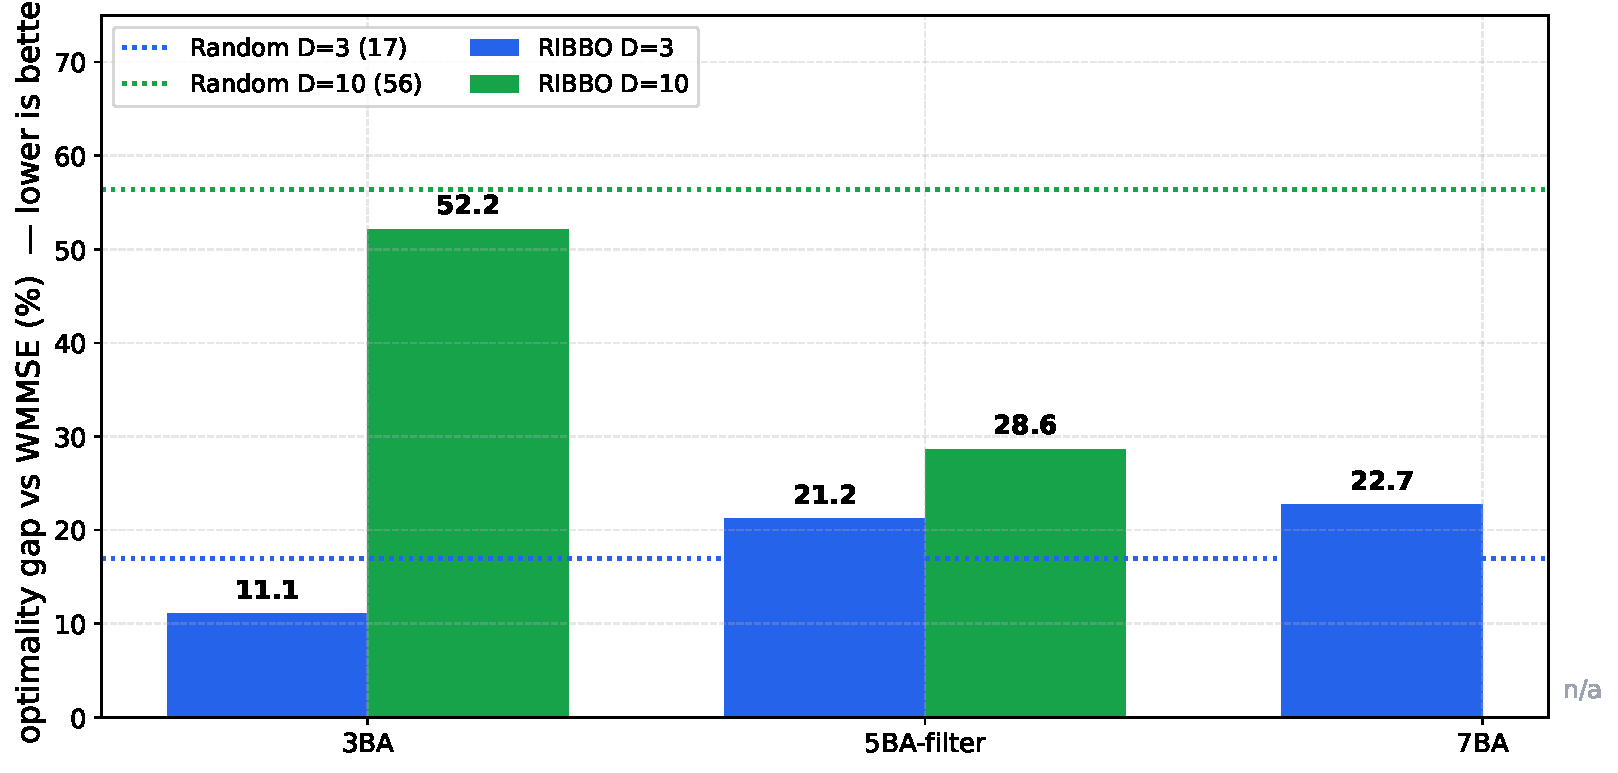
\includegraphics[width=\linewidth,height=0.66\textheight,keepaspectratio]{fig_ablation_2x2.pdf}
            \par\vspace{0.2em}{\scriptsize Bars: RIBBO gap to WMMSE.\, Dotted: Random.\, Lower $=$ better.}
        \end{column}
    \end{columns}
\end{frame}

% ----------------------------------------------------------------
% 4. SE vs EE (STAR slide)
% ----------------------------------------------------------------
\begin{frame}{Result 2 --- SE vs.\ EE: where RIBBO helps most \hfill {\small$\star$}}
    \small
    \begin{columns}[T,onlytextwidth]
        \begin{column}{0.40\textwidth}
            \textbf{EE's optimum is in the \emph{interior} (mid power), so uniform sampling rarely finds it}
            \par\vspace{0.3em}
            \scriptsize
            \begin{tabular}{lrrr}
                \toprule
                gap (\%) $\downarrow$ & RIBBO         & Random & $\Delta$        \\
                \midrule
                EE $D{=}3$            & \textbf{3.5}  & 17.2   & $13.7$          \\
                EE $D{=}10$           & \textbf{21.9} & 70.6   & $\mathbf{48.7}$ \\
                \midrule
                SE $D{=}10$           & 52.2          & 56.4   & $4.2$           \\
                \bottomrule
            \end{tabular}
            {\scriptsize\\ Same 3BA pool; only the reward changes. Separate model per reward and dimension. $\Delta=$ Random $-$ RIBBO.}

            \vspace{0.5em}
            \begin{tightitemize}
                \item On EE $D{=}10$, Random's gap stays at 71\% (uniform sampling rarely reaches the interior)
                \item RIBBO reduces it to 22\% --- a 48.7 pt smaller gap
                \item The clearest case for RIBBO in wireless
            \end{tightitemize}
        \end{column}
        \begin{column}{0.58\textwidth}
            \centering
            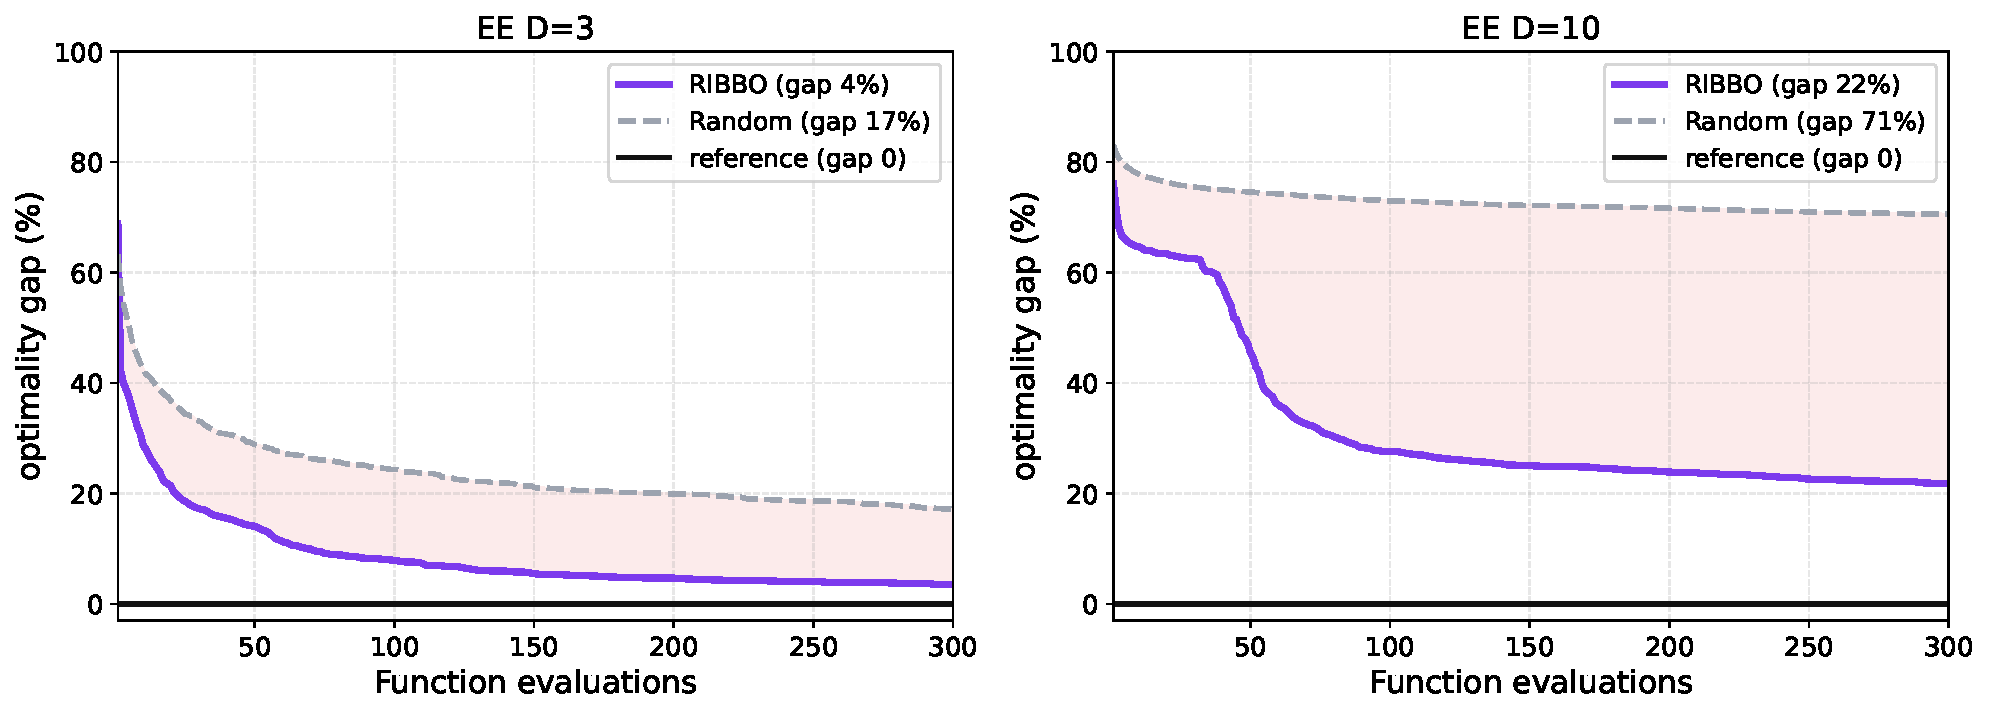
\includegraphics[width=\linewidth,height=0.66\textheight,keepaspectratio]{fig_ee_se.pdf}
            \par\vspace{0.2em}{\scriptsize Shaded $=$ how much smaller RIBBO's gap is; at $D{=}10$ Random's gap stays $\sim$71\%.}
        \end{column}
    \end{columns}
\end{frame}

% ----------------------------------------------------------------
% 5. Effect of dimension + recovery levers
% ----------------------------------------------------------------
\begin{frame}{Result 3 --- Effect of Problem Dimension (SE \& EE)}
    \small
    \begin{columns}[T,onlytextwidth]
        \begin{column}{0.40\textwidth}
            \textbf{Gap vs.\ dimension (SE \& EE, 3BA)}
            \begin{tightitemize}
                \item Gap grows with $D$ for both; one model \emph{per dimension} (not dimension-agnostic)
                \item RIBBO's EE $D{=}10$ gap $\ll$ Random (48.7 pts); SE difference small
            \end{tightitemize}
            \vspace{-0.1em}
            \textbf{Reducing the gap (SE):}
            \begin{tightitemize}
                \item Better algorithm choice: $D{=}20$ $67.0\to\mathbf{58.1}$ ($-8.9$)
                \item More steps: $D{=}10$ $27.1\to\mathbf{19.0}$ ($-8.1$)
                \item \emph{But} not for EE $D{=}20$ ($69.9\to69.7$) --- needs more data
            \end{tightitemize}
        \end{column}
        \begin{column}{0.58\textwidth}
            \centering
            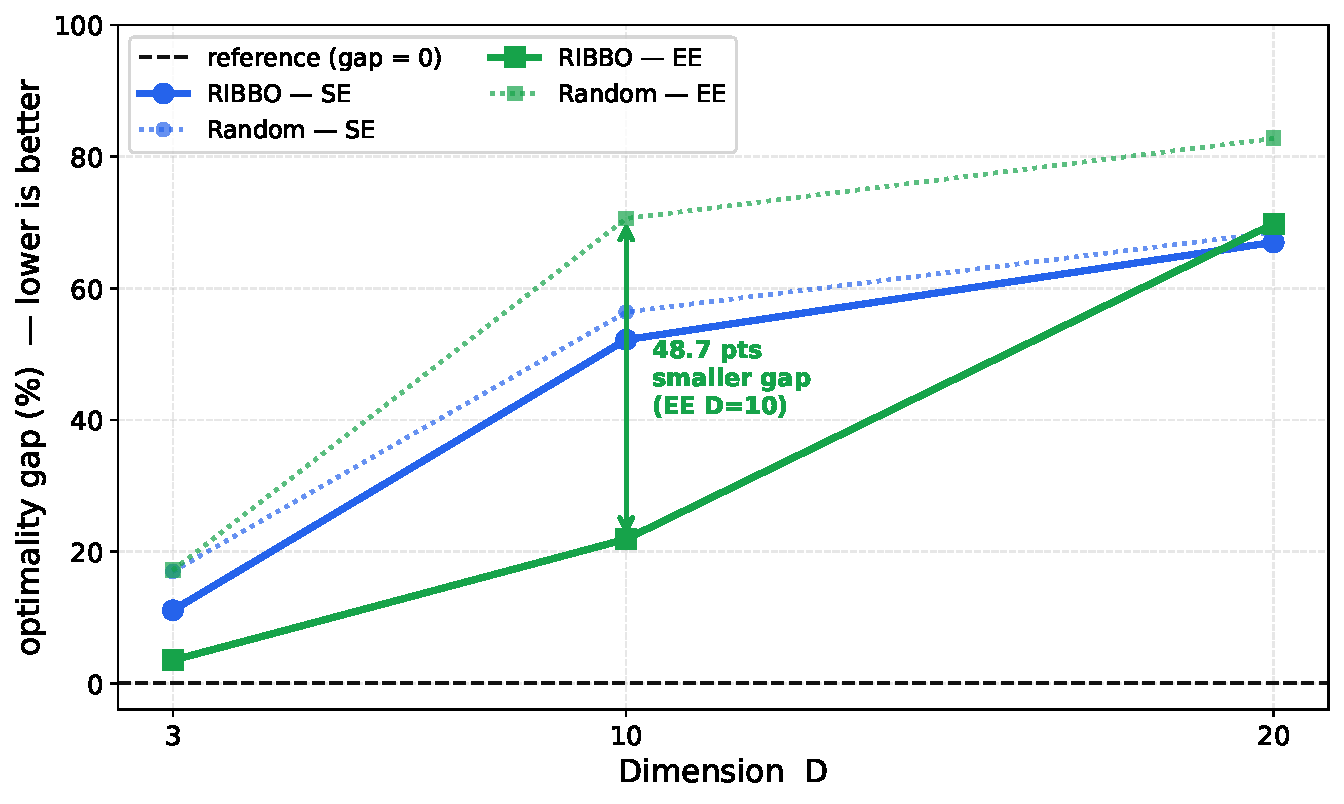
\includegraphics[width=\linewidth,height=0.66\textheight,keepaspectratio]{fig_synthesis.pdf}
        \end{column}
    \end{columns}
\end{frame}

% ----------------------------------------------------------------
% 5b. Robustness
% ----------------------------------------------------------------
\begin{frame}{Result 4 --- Robustness Checks}
    \small
    \begin{columns}[T,onlytextwidth]
        \begin{column}{0.46\textwidth}
            \begin{tightitemize}
                \item Random search ($=$ Lee et al.'s \emph{Brute-force} baseline) plateaus above a 50\% gap and rarely reaches the EE interior optimum; \textbf{RIBBO goes where uniform sampling cannot}
                \item Smaller gap than Random on \textbf{100\%} of channels at $D{=}10$ (SE \& EE), 99.5\% at $D{=}20$
                \item Statistically stable: 95\% CI $\pm{<}1.5$\% ($n{=}200$--$500$)
                \item EE advantage persists at $D{=}20$ (13 pt smaller, every channel)
                \item A local search reaches a $\sim$0 gap from \emph{any} start --- with the channel model / gradients the problem is easy, so RIBBO's value is the \emph{no-model} setting
            \end{tightitemize}
        \end{column}
        \begin{column}{0.46\textwidth}
            \centering
            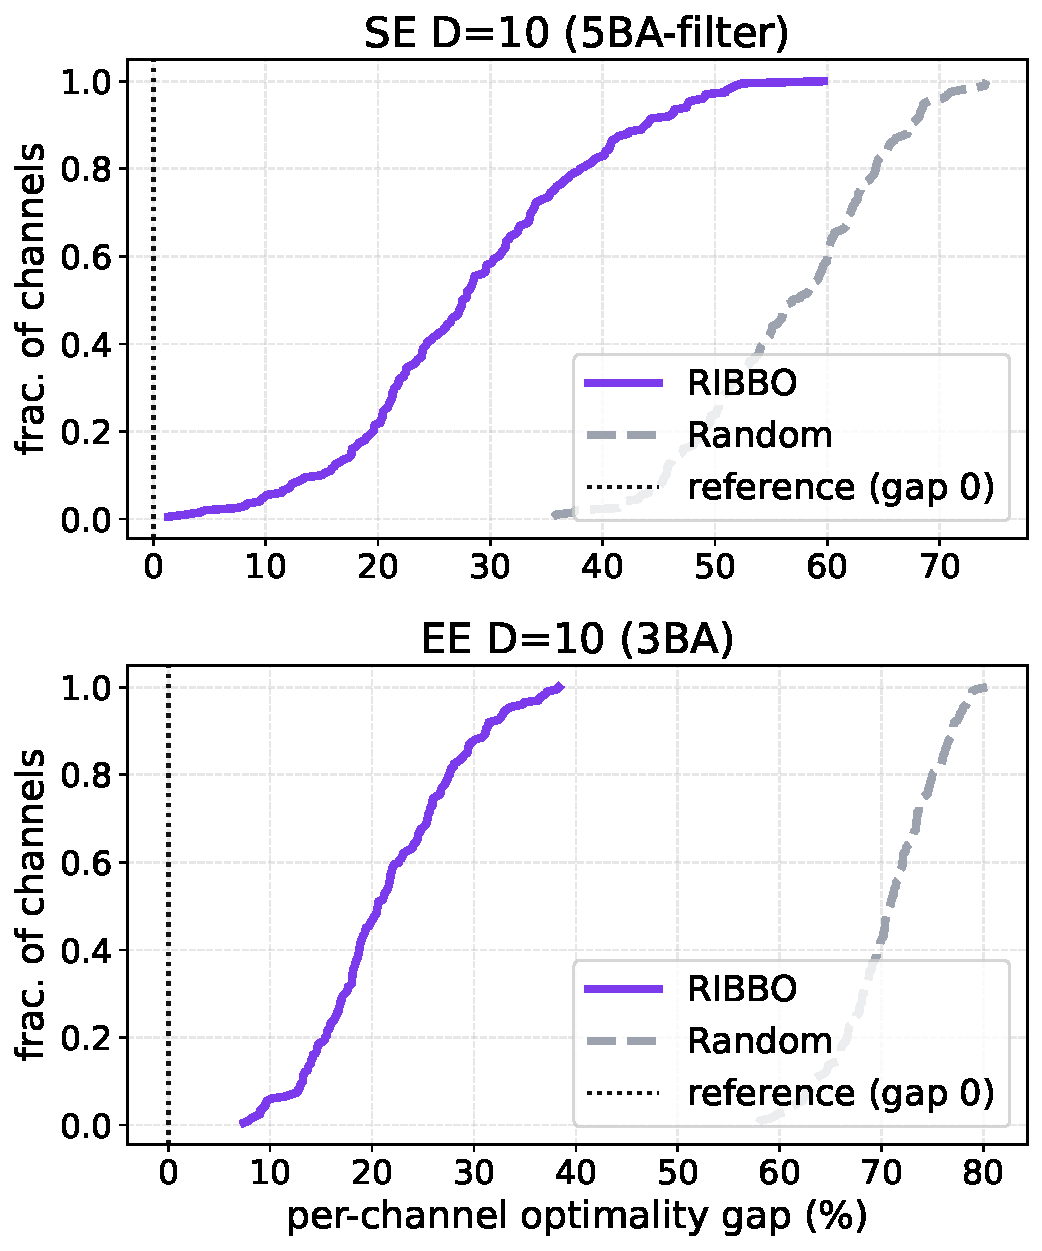
\includegraphics[width=\linewidth,height=0.86\textheight,keepaspectratio]{fig_per_channel.pdf}
        \end{column}
    \end{columns}
\end{frame}

% ----------------------------------------------------------------
% 6. Cross-domain transfer fails
% ----------------------------------------------------------------
\begin{frame}{Result 5 --- Training on Another Problem Doesn't Transfer}
    \small
    \begin{columns}[T,onlytextwidth]
        \begin{column}{0.42\textwidth}
            \textbf{Use a Rastrigin-trained model on IFC $D{=}10$ SE (no retraining)}
            \par\vspace{0.3em}
            \scriptsize
            \begin{tabular}{lr}
                \toprule
                Model                               & gap (\%) $\downarrow$ \\
                \midrule
                Rastrigin model, unchanged          & 68.2                  \\
                Rastrigin model, \textbf{rescaled}  & 68.8                  \\
                IFC model (reference)               & \textbf{55.1}         \\
                Random                              & $\sim$57              \\
                \bottomrule
            \end{tabular}

            \vspace{0.5em}
            \begin{tightitemize}
                \item Rescaling the target does \emph{not} help ($68.2\to68.8$)
                \item Our earlier guess (a scaling mismatch) was \textbf{wrong}
                \item Weak SE 3BA config here, so IFC-vs-Random is small --- the point is \emph{in-domain vs.\ transfer}
                \item $\Rightarrow$ \textbf{in-domain IFC training is needed}
            \end{tightitemize}
        \end{column}
        \begin{column}{0.56\textwidth}
            \centering
            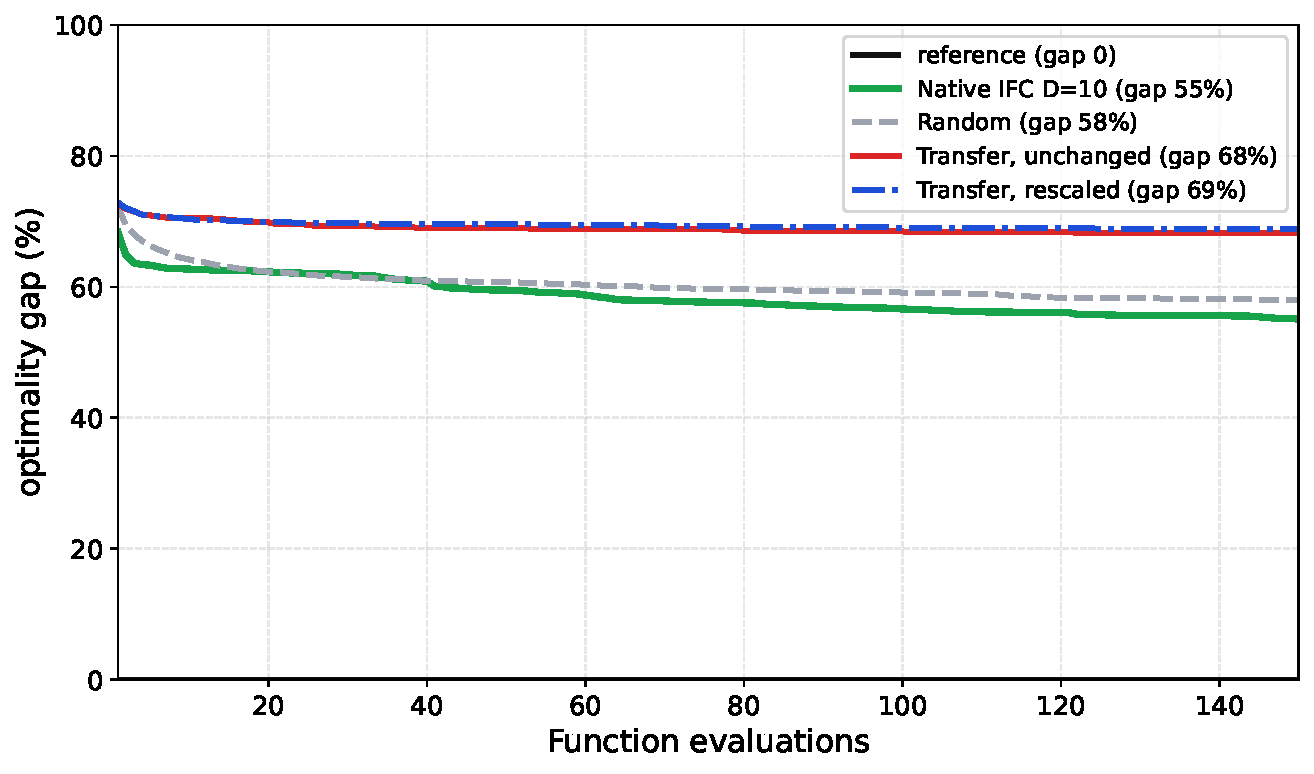
\includegraphics[width=\linewidth,height=0.64\textheight,keepaspectratio]{fig_transfer.pdf}
            \par\vspace{0.2em}{\scriptsize Rastrigin-trained (red/blue) have larger gaps than Random (gray); only IFC-trained (green) shrinks it.}
        \end{column}
    \end{columns}
\end{frame}

% ----------------------------------------------------------------
% 7. Insights
% ----------------------------------------------------------------
\section{Insights}

\begin{frame}{Insights --- When Does RIBBO Help?}
    \vspace{0.5em}
    \begin{itemize}
        \setlength{\itemsep}{0.9em}
        \item \textbf{The effect depends on the problem and its size.} For SE $D{=}3$ (on/off) simple methods already do well; for EE RIBBO shows a clearly smaller gap (48.7 pts at $D{=}10$).
        \item \textbf{Classical solvers need the channel model; RIBBO uses only scores.} WMMSE / fractional programming (FP) reach their reference solution with the model, and in our hybrid test a local search also closed the gap --- so RIBBO's clearest role is the \textbf{no-model} setting.
        \item \textbf{Which training algorithms help is problem-dependent.} Dropping weak ones reduced the SE gap at high $D$ ($-23.6$ pts) but increased the EE gap.
        \item \textbf{With a fixed setup, the gap grew with $D$;} more data / steps and a better algorithm choice reduced it (SE).
        \item \textbf{Cross-problem transfer did not work:} a Rastrigin-trained model did not improve on IFC; in-domain training was needed.
    \end{itemize}
\end{frame}

\end{document}
